
\subsection{Van het $x'y'z'$-assenstelstel naar het $xyz$-assenstelsel}
Het $x'y'z'$ assenstelsel wordt bekomen door het $xyz$-assenstelsel te roteren met een hoek $\alpha$ rond de x-as. De omgekeerde transformatie draait dus met een negatieve hoek $\alpha$ rond de x-as. Het $x''y''z''$-assenstelsel heeft dezelfde ori\"entatie als het $x'y'z'$-assenstelsel. Hun transformatiematrices zijn daarom hetzelfde.

\begin{figure}[H]
\centering
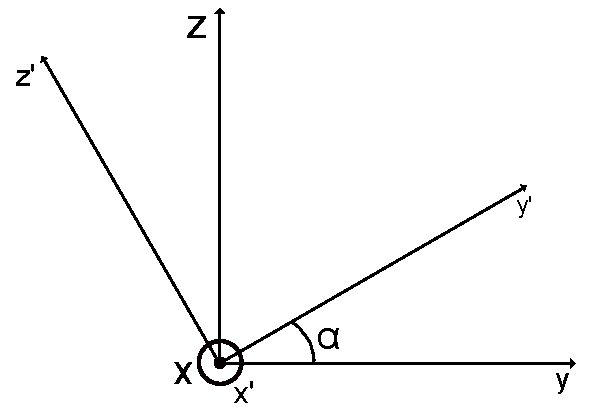
\includegraphics[scale=0.5]{x'y'z'.pdf}
\caption{Het $x'y'z'$-assenstelsel}
\end{figure}

\begin{equation*}
R^{x'y'z' \rightarrow xyz}=
  \begin{bmatrix}
    1 & 0 & 0\\
    0 & \cos(\alpha) & -\sin{\alpha}\\ 
    0 & \sin{\alpha} & \cos(\alpha)\
    \end{bmatrix}
\end{equation*}



\subsection{Van het $x'''y'''z'''$-assenstelsel naar het $x''y''z''$-assenstelsel}
Het $x'''y'''z'''$-assenstelsel wordt bekomen door het $x''y''z''$-assenstelsel te roteren met een hoek $\beta$ rond de $y''$-as. De transformatiematrix draait dus met een negatieve hoek $\beta$ rond de $y'''$-as. Deze transformatiematrix kan ook gebruikt worden om co\"ordinaten naar het $x'y'z'$-assenstelsel te converteren. De ori\"entatie van het $x'y'z'$-assentstelsel en van het $x''y''z''$-assenstelsel is immers hetzelfde.

\begin{figure}[H]
\centering
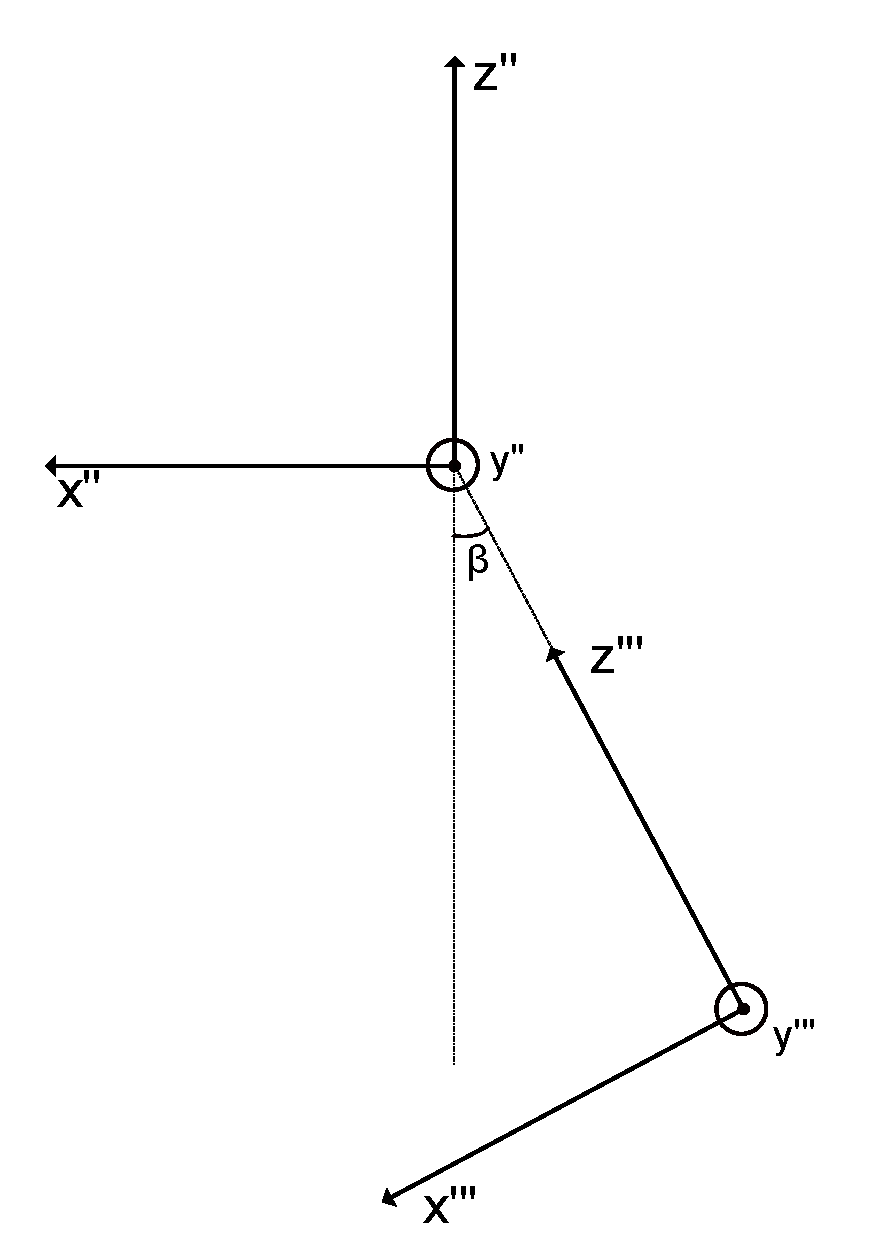
\includegraphics[scale=0.35]{x'''y'''z'''.pdf}
\caption{Het $x'''y'''z'''$-assenstelsel}
\end{figure}

\begin{equation*}
R^{x'''y'''z''' \rightarrow x''y''z''}=
  \begin{bmatrix}
    \cos(\beta) & 0 & sin(\beta)\\
    0 & 1 & 0\\ 
    -\sin(\beta) & 0 & \cos(\beta)\
    \end{bmatrix}
\end{equation*}

Voor de omgekeerde transformatie wordt deze matrix ge\"inverteerd.
\begin{equation*}
R^{x''y''z'' \rightarrow x'''y'''z'''}=
  \begin{bmatrix}
    \cos(\beta) & 0 & -sin(\beta)\\
    0 & 1 & 0\\ 
    \sin(\beta) & 0 & \cos(\beta)\
    \end{bmatrix}
\end{equation*}


\subsection{Van het $x'''y'''z'''$-assenstelsel naar het $xyz$-assenstelsel}
Om van het $x'''y'''z'''$-assenstelsel naar het $xyz$-assenstelsel te gaan, worden de vorige twee berekende transformatiematrices met elkaar vermenigvuldigd. Eerst worden de $x'''y'''z'''$-co\"ordinaten getransformeerd naar het $x''y''z''$-assenstelsel. Vervolgens worden ze omgezet naar het $xyz$-assenstelsel.
\begin{equation*}
\begin{split}
R^{x'''y'''z''' \rightarrow xyz} & =R^{x'''y'''z''' \rightarrow x''y''z''}R^{x'y'z' \rightarrow xyz} \\
&=
  \begin{bmatrix}
      1 & 0 & 0\\
      0 & \cos(\alpha) & -\sin{\alpha}\\ 
      0 & \sin{\alpha} & \cos(\alpha)\
      \end{bmatrix}
  \begin{bmatrix}
      \cos(\beta) & 0 & sin(\beta)\\
      0 & 1 & 0\\ 
      -\sin(\beta) & 0 & \cos(\beta)\
      \end{bmatrix} \\
&=
  \begin{bmatrix}
      \cos(\beta) & 0 & \sin(\beta)\\
      \sin(\alpha)\sin(\beta) & \cos(\alpha) & -\sin(\alpha)\cos(\beta)\\
      -\cos(\alpha)\sin(\beta) & \sin(\alpha) & \cos(\alpha)\cos(\beta)\  
      \end{bmatrix}
\end{split}
\end{equation*}